\newpage
\section{Mögliche Aspekte}
\subsection{Persönliche mobile Arbeitsumgebung}
Heutzutage werden Computer für alle möglichen Tätigkeiten in der Arbeitswelt benötigt, ob nun für kleinere Aufgaben oder für komplexe Berechnung mit Hilfe eines am Netzwerk angeschlossenen Supercomputers. In einer modernen Umgebung kann es unter Umständen notwendig sein den Arbeitsplatz aufgrund einer Tätigkeit zu wechseln um diese ausführen zu können. Dies hat allerdings zur Folge, dass dort der eigene Rechner mit den zugehörigen Daten und möglicherweise auch die benötigte Rechenleistung nicht verfügbar ist.
Um für die Benutzer eine auf allen Rechnersystemen einheitliche Bedienerfahrung gewährleisten zu können, lässt sich eine sogenannte mobile personalisierte virtuelle Computerumgebung (MOVE)\nomenclature{MOVE}{Mobile Personalized Virtual Computing Environment} nutzen. Durch diese Umgebung wird dem Benutzer auf jeder beliebigen Maschine eine gleichmäßig konsistente Desktop-Rechner-Umgebung präsentiert, welche sowohl die gleichen personenbezogenen Daten und Software als auch die verfügbare Rechenleistung liefert wie am eigenen Arbeitsplatzrechner. Eine solche Desktop-Rechner-Umgebung besteht zum Großteil aus der installierten Software einschließlich des Betriebs- und Dateisystems. Diese könnten zwar vom Speichermedium auf ein anderes übertragen werden, aufgrund der engen Koppelung ließe sich diese allerdings nicht einfach auf einem neuen System ausführen. Um diese Abstraktion gewährleisten zu können, wird die Technologie der virtuellen Maschinen (VM)\nomenclature{VM}{Virtual Maschine} genutzt.\footcite[Vgl.][Seite 890 f.]{MOVE}

Bei der Virtualisierung werden mit Hilfe von Technologien die Ressourcen eines Rechnersystems auf mehrere einzelne Klienten aufgeteilt um diese effektiver und flexibler nutzbar zu machen. Dies geschieht dadurch, dass unterschiedliche Klassen von Anwendungen auf wenigen physischen Systemen konsolidiert und von mehreren unabhängigen Betriebssysteminstanzen gleichzeitig genutzt werden können.\footcite[Vgl.][Seite 197]{InformatikSpektrum} Diese Virtualisierung wird mit der Hypervisor Technologie implementiert. Ein Hypervisor, oder auch Virtual Maschine Monitor (VMM)\nomenclature{VMM}{Virtual Maschine Monitor} genannt, ist ein Stück Hardware oder Software welches Systemressourcen virtualisiert, wobei zwischen Typ 1 und Typ 2 Hypervisors unterschieden wird. Typ 1 Hypervisors sind direkt auf der Hardware implementiert, Typ 2 Hypervisors laufen dagegen auf einem Host Betriebssystem. Dieses stellt Dienste wie Speichermanagement zur Virtualisierung zur Verfügung.\footcite[Vgl.][]{ibm}

\begin{figure}[H]
\begin{center}
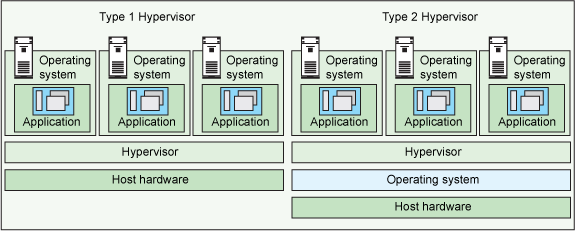
\includegraphics[width=0.9\textwidth]{hypervisors}
\caption{Unterschiede zwischen den Typ 1 und Typ 2 Hypervisors}
Quelle: \cite[]{ibm}
\end{center}
\end{figure}
\vspace{-1cm}